\chapter{Experimentation}
\label{ch_experimentation}
%This is a chapter added into the template because Dr Winberg's example reports have it.
The following experiments were developed to evaluate the laser tag system. The objective of these experiments is to assess the performance and characteristics of the modules and software developed during the design phase.

The experiments may be separated into two categories, those evaluating specific modules and those evaluating software algorithms. Outside these categories is the system performance experiment which evaluates the combined behaviour of the modules and software by means of a range test.

\begin{figure}[H]
	\centering
	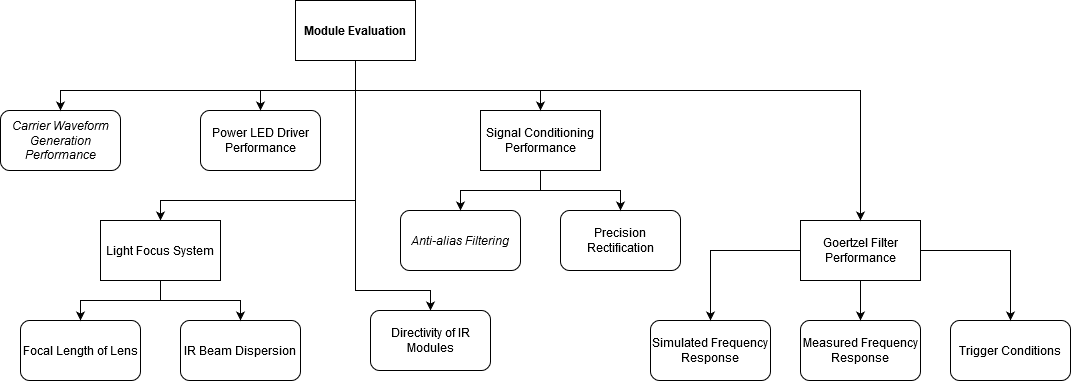
\includegraphics[width=\linewidth]{figures/experimentation/experiments_overview_module_evaluation.png}
	\captionof{figure}{Overview - Module Specific Experiemnts}
	\label{fig:experiments_overview_module_evaluation}
\end{figure}

\begin{figure}[H]
	\centering
	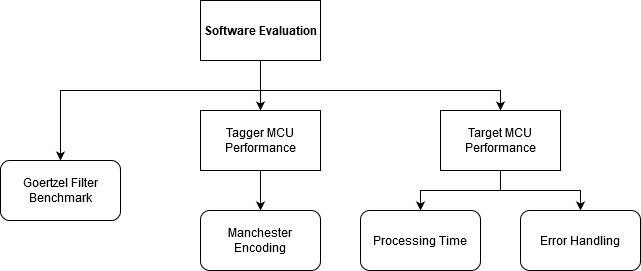
\includegraphics[width=.7\linewidth]{figures/experimentation/experiments_overview_software_evaluation.png}
	\captionof{figure}{Overview - Software Specific Experiemnts}
	\label{fig:experiments_overview_software_evaluation}
\end{figure}

In figures \ref{fig:experiments_overview_module_evaluation} and \ref{fig:experiments_overview_software_evaluation} above, a rectangle with rounded edges indicates an experiment while rectangles with sharp edges indicate categories.




%%%%%%%%%%%%%%%%%%%%%%%%%%%%%%%%%%%%%%%%%%%
%%%%%%%%%%%%%%%%%%%%%%%%%%%%%%%%%%%%%%%%%%%



\section{Module Evaluation}

\subsection{Carrier Waveform Generation Performance}
The carrier waveform module was tested under two conditions. Initially a constant high logic signal was presented at the input to evaluate the steady-state frequency generation. Following this a Manchester transmission was presented at the input and the output waveform was traced.

The output of the carrier waveform generation module is an open-collector, thus a pull-up resistor was used to allow the oscilloscope to distinguish between the output states. An oscilloscope was used to trace both the input and output waveforms. The experimental setup is illustrated in figure \ref{fig:carrier_generation_module_experiment_setup}

\begin{figure}[H]
	\centering
	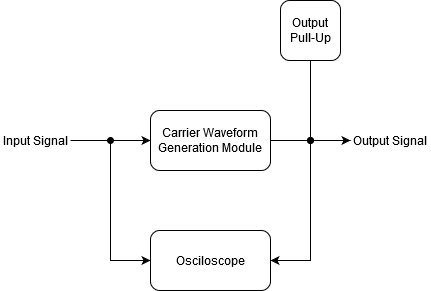
\includegraphics[width=.5\linewidth]{figures/experimentation/carrier_generation_module_experiment.png}
	\captionof{figure}{Experimental Setup - Carrier Waveform Generation Module}
	\label{fig:carrier_generation_module_experiment_setup}
\end{figure}

The steady-state response was measured after the input had been brought high for approximately 1 second. During the Manchester transmission, tones were generated for periods less than 2mS.


%%%%%%%%%%%%%%%%%%%%%%%%%%%%%%%%%%%%%%%%%%%



\subsection{Power LED Driver Performance}

The LED driver module must be capable of modulating a high-power IR led at a frequency of 36kHz.

To verify that the power LED driver module operates as expected and to evaluate the module's performance, a set of test input frequencies were injected and the response recorded. Figure \ref{fig:power_led_driver_experiemnet_setup} illustrates the experimental setup.

\begin{figure}[H]
	\centering
	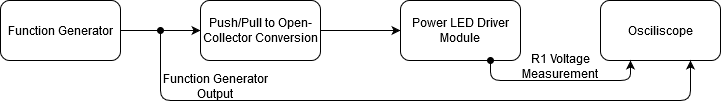
\includegraphics[width=.9\linewidth]{figures/experimentation/power_led_driver_experimental_setup.png}
	\captionof{figure}{Experimental Setup - Power LED Driver}
	\label{fig:power_led_driver_experiemnet_setup}
\end{figure}

Each test input was generated as a square wave using a function generator and converted to an open-collector signal before being injected into the driver module. To monitor the LED's state, an oscilloscope was connected across the shunt resistor R1 (see schematic in figure \ref{fig:schematic_power_led_driver}). Monitoring the resistor provided insight into both the state of the LED and the current through the LED. The current flowing through the power LED was calculated using Ohms law. \(I_{led} = \frac{V_{R1}}{0.68\Omega}\).



%%%%%%%%%%%%%%%%%%%%%%%%%%%%%%%%%%%%%%%%%%%



\subsection{Light Focus System}
\subsubsection{Focal Length of Lens}
\label{exp:focal_length}

The following experiment was performed to determine the focal length of the lens so that the dimensions of the light focus system could be determined.

Figure \ref{fig:focal_length_experiemnt} shows the experimental setup used to determine the focal length of the lens. The lens was secured using a circuit board holder to allow for precise adjustment of height above the working surface. A light source was placed directly above the lens at a distance of 1.2m.

\begin{figure}[H]
	\centering
	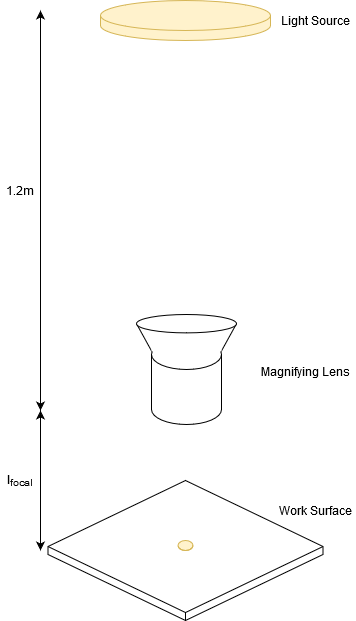
\includegraphics[width=.4\linewidth]{figures/experimentation/focal_length.png}
	\captionof{figure}{Focal Length Experiment Setup}
	\label{fig:focal_length_experiemnt}
\end{figure}

After setting up the experiment, the lens was slowly adjusted along the vertical axis until the spot formed on the work surface was a minimum size. A tape measure was used to find the distance from the work surface to the lens.

\subsubsection{Beam Dispersion}

To evaluate the light focusing tube, two different power LEDs where used, a 3W white (visible light) power LED and a 3W IR power LED. Experimenting with a white LED allowed a set of measurements to be taken without the use of an intermediary tool, as was necessary when measuring the IR beam spot diameter.

\begin{figure}[H]
	\centering
	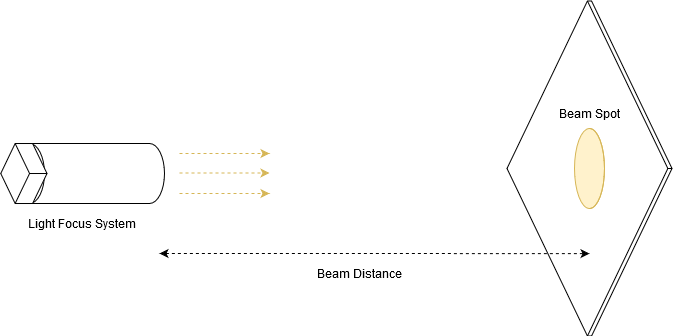
\includegraphics[width=.7\linewidth]{figures/experimentation/beam_spot_experiement.png}
	\captionof{figure}{Light Focus System Experiment Setup}
	\label{fig:focus_system_experiemnt}
\end{figure}

Figure \ref{fig:focus_system_experiemnt} above shows the experimental setup.

In both cases, the focus system was set up some distance from a flat surface. The light was powered and after marking the edge of the beam spot the diameter was measured. Each diameter was recorded along with the beam distance. A video camera in 'night shot' mode was used to find and mark the edge of the IR beam spot.



%%%%%%%%%%%%%%%%%%%%%%%%%%%%%%%%%%%%%%%%%%%


\subsection{Directivity of Detector Modules}

To characterise the directivity of the photodiode and phototransistor detector modules, the following experiment was performed.

\begin{figure}[H]
	\centering
	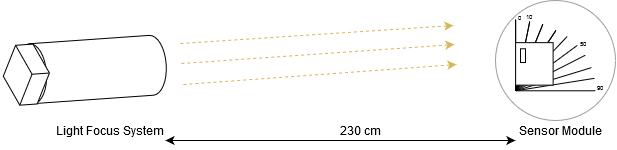
\includegraphics[width=.9\linewidth]{figures/experimentation/beam_angle_of_receiver.png}
	\captionof{figure}{Directivity Experimental Setup}
	\label{fig:directivity_experiement_setup}
\end{figure}

The light focus system was connected to the LED driver module which was modulated at 36kHz by the carrier waveform generator module. The modulated beam was then aimed at the sensor module, placed 230cm away. The output of the detector module was connected to an oscilloscope to trace the output waveform.

The IR beam was positioned off centre so that when the module was adjusted to have an indecent angle of 0\textdegree{} the output of the sensor module was only just saturating, this ensured the sensitivity could be accurately tracked.

Starting with a 0\textdegree{} angle of incidence, the module was rotated in increments of 10\textdegree{} until the angle of incidence was equal to 90\textdegree. After each increment the output waveform was exported for processing in Octave.

Octave was used to calculate the RMS\footnote{root mean square} voltages for the recorded output waveforms. The RMS values were normalized and plotted to visualize each module's directivity.

The IR receiver module was tested following the same experimental method, however, because the output of this module is a logic level, sensitivity cannot be measured.




%%%%%%%%%%%%%%%%%%%%%%%%%%%%%%%%%%%%%%%%%%%


\subsection{Signal Conditioning Performance}

\subsubsection{Anti-alias Filtering}
To evaluate the anti-aliasing filter, a 36kHz square waveform with an amplitude of 2V was generated at the input of the signal conditioning module. An oscilloscope was used to compare this input waveform with the waveform at the output of the filter.

\subsubsection{Precision Rectification}
To evaluate the precision rectifier, a function generator was used to inject a 36kHz square wave with an amplitude of 2V into the signal conditioning module. An oscilloscope was used to trace the waveform at both the input and output points of the precision rectifier.


%%%%%%%%%%%%%%%%%%%%%%%%%%%%%%%%%%%%%%%%%%%




\subsection{Goertzel Filter Performance}

To evaluate the performance of the Goertzel filter the following experiments where performed.

\begin{itemize}
	\item Simulated Frequency Response
	\item Measured Frequency Response
	\item Trigger Conditions
\end{itemize}

\subsubsection{Simulated Frequency Response}
The expected frequency response was simulated using the Octave\footnote{Open-source alternative to Matlab} environment. This was achieved by implementing an identical algorithm as the one implemented on the STM32. This optimized implementation of the Goertzel algorithm is presented in listing \ref{lst:optimized_goertzel_algorithm}.
%This function is optimized according to the design outlined in section \ref{sec:filter_optimization_design} and the value returned by the function is the magnitude of the DFT coefficient squared.

A second Octave script was written to find the filter response (see listing \ref{lst:frequency_response_script}). This script generated a range of frequencies in the form of sampled sin waves over the range of 0Hz to 71.7kHz with an interval of 100Hz. The test tones were scaled, off-set and sampled to match the conversion values that would be returned by the ADC onboard the STM32F0. Each generated tone was processed by the Octave Goertzel filter.
%todo: this next part is bloated
%After generating each frequency, the above-mentioned Octave implementation of the Goertzel filter was called and the computation result stored. An example, 36kHz waveform is given in the appendix, figure \ref{fig:sampled_36khz_sinusoid}.

After passing each tone through the filter, the results were plotted to reveal the frequency response of the algorithm. The frequency response was simulated for tones with an amplitude of both 500mV and 1V.

\subsubsection{Measured Frequency Response}
%todo: rework this methodology wording
%The next experiment involved testing the Goertzel filter to check that the filter implementation was working as expected. This was done by generating a sinusoid waveform at the input to the ADC and using the serial communication port to transfer the value of the Goertzel filtering result.

To test the actual frequency response of the tone decoder module, a set of tones were generated using a function generator and placed at the input to the tone decoder module. A serial communication channel was used transfer the processed results for analysis.

The function generator was manually configured for each test frequency and a button was used to initiate each transfer of the algorithm's output.

The first tone generated was 1kHz, the frequency was then incremented in 3kHz steps until a tone of 70kHz was reached. The results were processed by Octave to generate a plot and compare the empirical and simulated responses.


\subsubsection{Trigger Conditions}
%todo: consider more concise wording
%To evaluate the high-level functionality of the Goertzel, an experiment was performed to determine the amplitude and frequency boundary pairs which cause the Goertzel filter to trigger.

No automatic gain control is integrated into the Goertzel algorithm, there is therefore a minimum signal amplitude required to trigger the output. This experiment was performed to gain insight into this minimum amplitude and how that amplitude changes as the frequency moves away from the centre frequency of 36kHz.

A function generator was connected to the input of the Goertzel filter module and an oscilloscope used to monitor both the input and output waveforms. Throughout the experiment, the generated sinusoidal waveform was offset by 1V to ensure the input voltage remained positive.

Initially the amplitude of a 36kHz tone was manually adjusted to determine the smallest amplitude at which the Goertzel filter would trigger. This occurs at around 297mV.

The amplitude of the generated input tone was initially set to 300mV and then increased in  50mV increments to 500mV. For each amplitude, the function generator was configured to sweep though all frequencies between 28kHz and 44kHz. The oscilloscope was then used to find the frequencies which caused the output of the Goertzel filter to trigger. For every amplitude value, both the upper and lower frequency boundaries were recorded.

These results were plotted using Octave.





%%%%%%%%%%%%%%%%%%%%%%%%%%%%%%%%%%%%%%%%%%%
%%%%%%%%%%%%%%%%%%%%%%%%%%%%%%%%%%%%%%%%%%%






%%%%%%%%%%%%%%%%%%%%%%%%%%%%%%%%%%%%%%%%%%%
%%%%%%%%%%%%%%%%%%%%%%%%%%%%%%%%%%%%%%%%%%%

\section{Software Evaluation}






\subsection{Goertzel Filter Benchmark}
%todo: this can surely be made shorter
The following experiment was performed to give insight into the effects of increasing the number of samples (N) and optimizing the algorithm by reducing the number of multiplications. %This was done to measure the benefits to be gained from the two optimization methods and the effectiveness of these methods.

To measure the unoptimized performance, the Goertzel algorithm (see listing \ref{lst:goertzel_algorithm}) was implemented inside the circular buffer's callback functions. This implementation will be referred to as the unoptimized algorithm. As a consequence of using a circular buffer with two segments, there are two callback functions. The Goertzel implementations used inside both callback functions are identical, with the only exception being the location in the buffer from which samples are read.

The timing was measured externally using an oscilloscope. Just before the Goertzel algorithm began executing an LED was turned on using one of the GPIO pins. This LED was turned off as soon as the algorithm finished executing. Each of the two callback functions used a unique GPIO pin to toggle separate LEDs. Figure \ref{fig:goertzel_optimization_experiemnt} below illustrates the experimental setup in the form of a block diagram.

\begin{figure}[H]
	\centering
	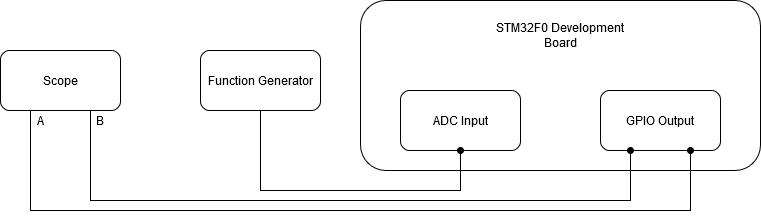
\includegraphics[width=.9\linewidth]{figures/experimentation/goertzel_speed_test_diagram.png}
	\captionof{figure}{Goertzel Optimization Experimental Setup}
	\label{fig:goertzel_optimization_experiemnt}
\end{figure}

A signal generator was used to produce a 36kHz tone with an amplitude of 1V and an offset of 1V. Using a 36kHz waveform ensured that the filter had to compute large multiplications, providing insight into performance under the most demanding circumstances.

The experiment was broken into iterations, each iteration began by setting N to the desired number of samples, following this the code was compiled and executed on the development board. The signal generator was attached and enabled and the scope probes were attached to the GPIO pins responsible for timing. The scope was adjusted so that between 20 and 30 pulses were traced. 

The independent variable N (number of samples to process) was set to 4 for the first iteration and doubled for each consecutive iteration until a value of 64 was reached. These five values of N all preserve the integer ratio required by equation \ref{eqn:k_N_and_fb_fs_ratio}.

Using the measurement tools built into the Picoscope software the 'high pulse width' for the GPIO pin outputs were averaged, along with the average duty cycle of those waveforms. Only the results from the timing of the first callback function were recorded, the results from the second callback timing waveform was used as a sanity check to ensure both waveforms were practically identical.

%For this experiment, only the trace of the callback responsible for the first half of the circular buffer being full was recorded. The timing for the second half of the buffer being full was used only as a sanity check, both the callback functions should run for the same amount of time as each is executing the same algorithm, therefore, the average high pulse width for each should be the same.

After the experiment was run for all 5 iterations, the unnecessary multiplications (as discussed in section \ref{sec:filter_optimization_design}) were removed from the Goertzel implementation and the above experimental process repeated with the optimized algorithm.



%%%%%%%%%%%%%%%%%%%%%%%%%%%%%%%%%%%%%%%%%%%




\subsection{Tagger MCU Performance}

\subsubsection{Manchester Encoding}
To validate the Manchester encoding functionality of the tagger, an oscilloscope was connected to the GPIO responsible for generating the Manchester waveforms.

The tagger MCU was set to generate transmissions containing the value of a counter which incremented after each transmission. The oscilloscope traces were evaluated to confirm valid encoding and timing according to the design specifications.

%%%%%%%%%%%%%%%%%%%%%%%%%%%%%%%%%%%%%%%%%%%



\subsection{Target MCU Performance}

In both of the following experiments, the receiver's code was modified to set a GPIO pin high at the beginning of the Manchester decoding function call and reset the pin after the decoding completes. The tagger MCU was wired directly to the target MCU to mitigate external factors.

\subsubsection{Processing Time}
\label{sec:processing_time_experiment}
%todo: consider more concise
The processing time taken by the state machine to decode Manchester waveforms is affected by the contents of the transmission, this is because the number of transitions depends on the encoded bit-stream. The following experiment set out to measure the varying computation times of the decoding process.

Three data packets were chosen, based on the corresponding number of edges in the Manchester encoded sequence. The lowest possible number of edges in a valid message is 20 while the highest is 36. The middle message with the data value 11111 was chosen arbitrarily as a third test case.

\begin{table}[H]
	\centering
	\begin{tabular}{ccc}
		\hline
		\textbf{\begin{tabular}[c]{@{}c@{}}15-Bit Data\\ (Decimal)\end{tabular}} & \textbf{\begin{tabular}[c]{@{}c@{}}18-bit Transmission\\ (Hexadecimal)\end{tabular}} & \textbf{Number of Edges} \\ \hline
		10922 & 0x2AAAB & 20 \\ \hline
		11111 & 0x2AD9F & 26 \\ \hline
		32767 & 0x3FFFF & 36 \\ \hline
	\end{tabular}
\end{table}

An oscilloscope was used to trace the state of the GPIO pin used to indicate the when the decoding function was executing. A second probe was used to trace the incoming Manchester waveform, this allowed the length of the timeout period to be measured as well.

\subsubsection{Error Handling}
To validate the error handling capabilities of the target, two different error conditions where simulated. In each case, the Manchester input sequence and the GPIO pin (used to indicate when the decoding function was executing) were traced by an oscilloscope.

The first error condition was generated by transmitting Manchester encoded messages with a delay of 20mS between transmissions (a period shorter than the processing time). The second error condition was generated by continuously transmitting messages without any period between them.



%%%%%%%%%%%%%%%%%%%%%%%%%%%%%%%%%%%%%%%%%%%
%%%%%%%%%%%%%%%%%%%%%%%%%%%%%%%%%%%%%%%%%%%




%%%%%%%%%%%%%%%%%%%%%%%%%%%%%%%%%%%%%%%%%%%
%%%%%%%%%%%%%%%%%%%%%%%%%%%%%%%%%%%%%%%%%%%

\section{System Range}

To determine the range of the laser tag system, the system was set up on a large open space. The tagger and target were set up on two small tables. The target subsystem was moved relative to the tagger subsystem to adjust the transmission range. To measure the impact of ambient lighting on the system the experiment was performed during the afternoon several hours before sunset and several hours after sunset.

\begin{figure}[H]
	\centering
	\begin{minipage}{.48\textwidth}
		\centering
		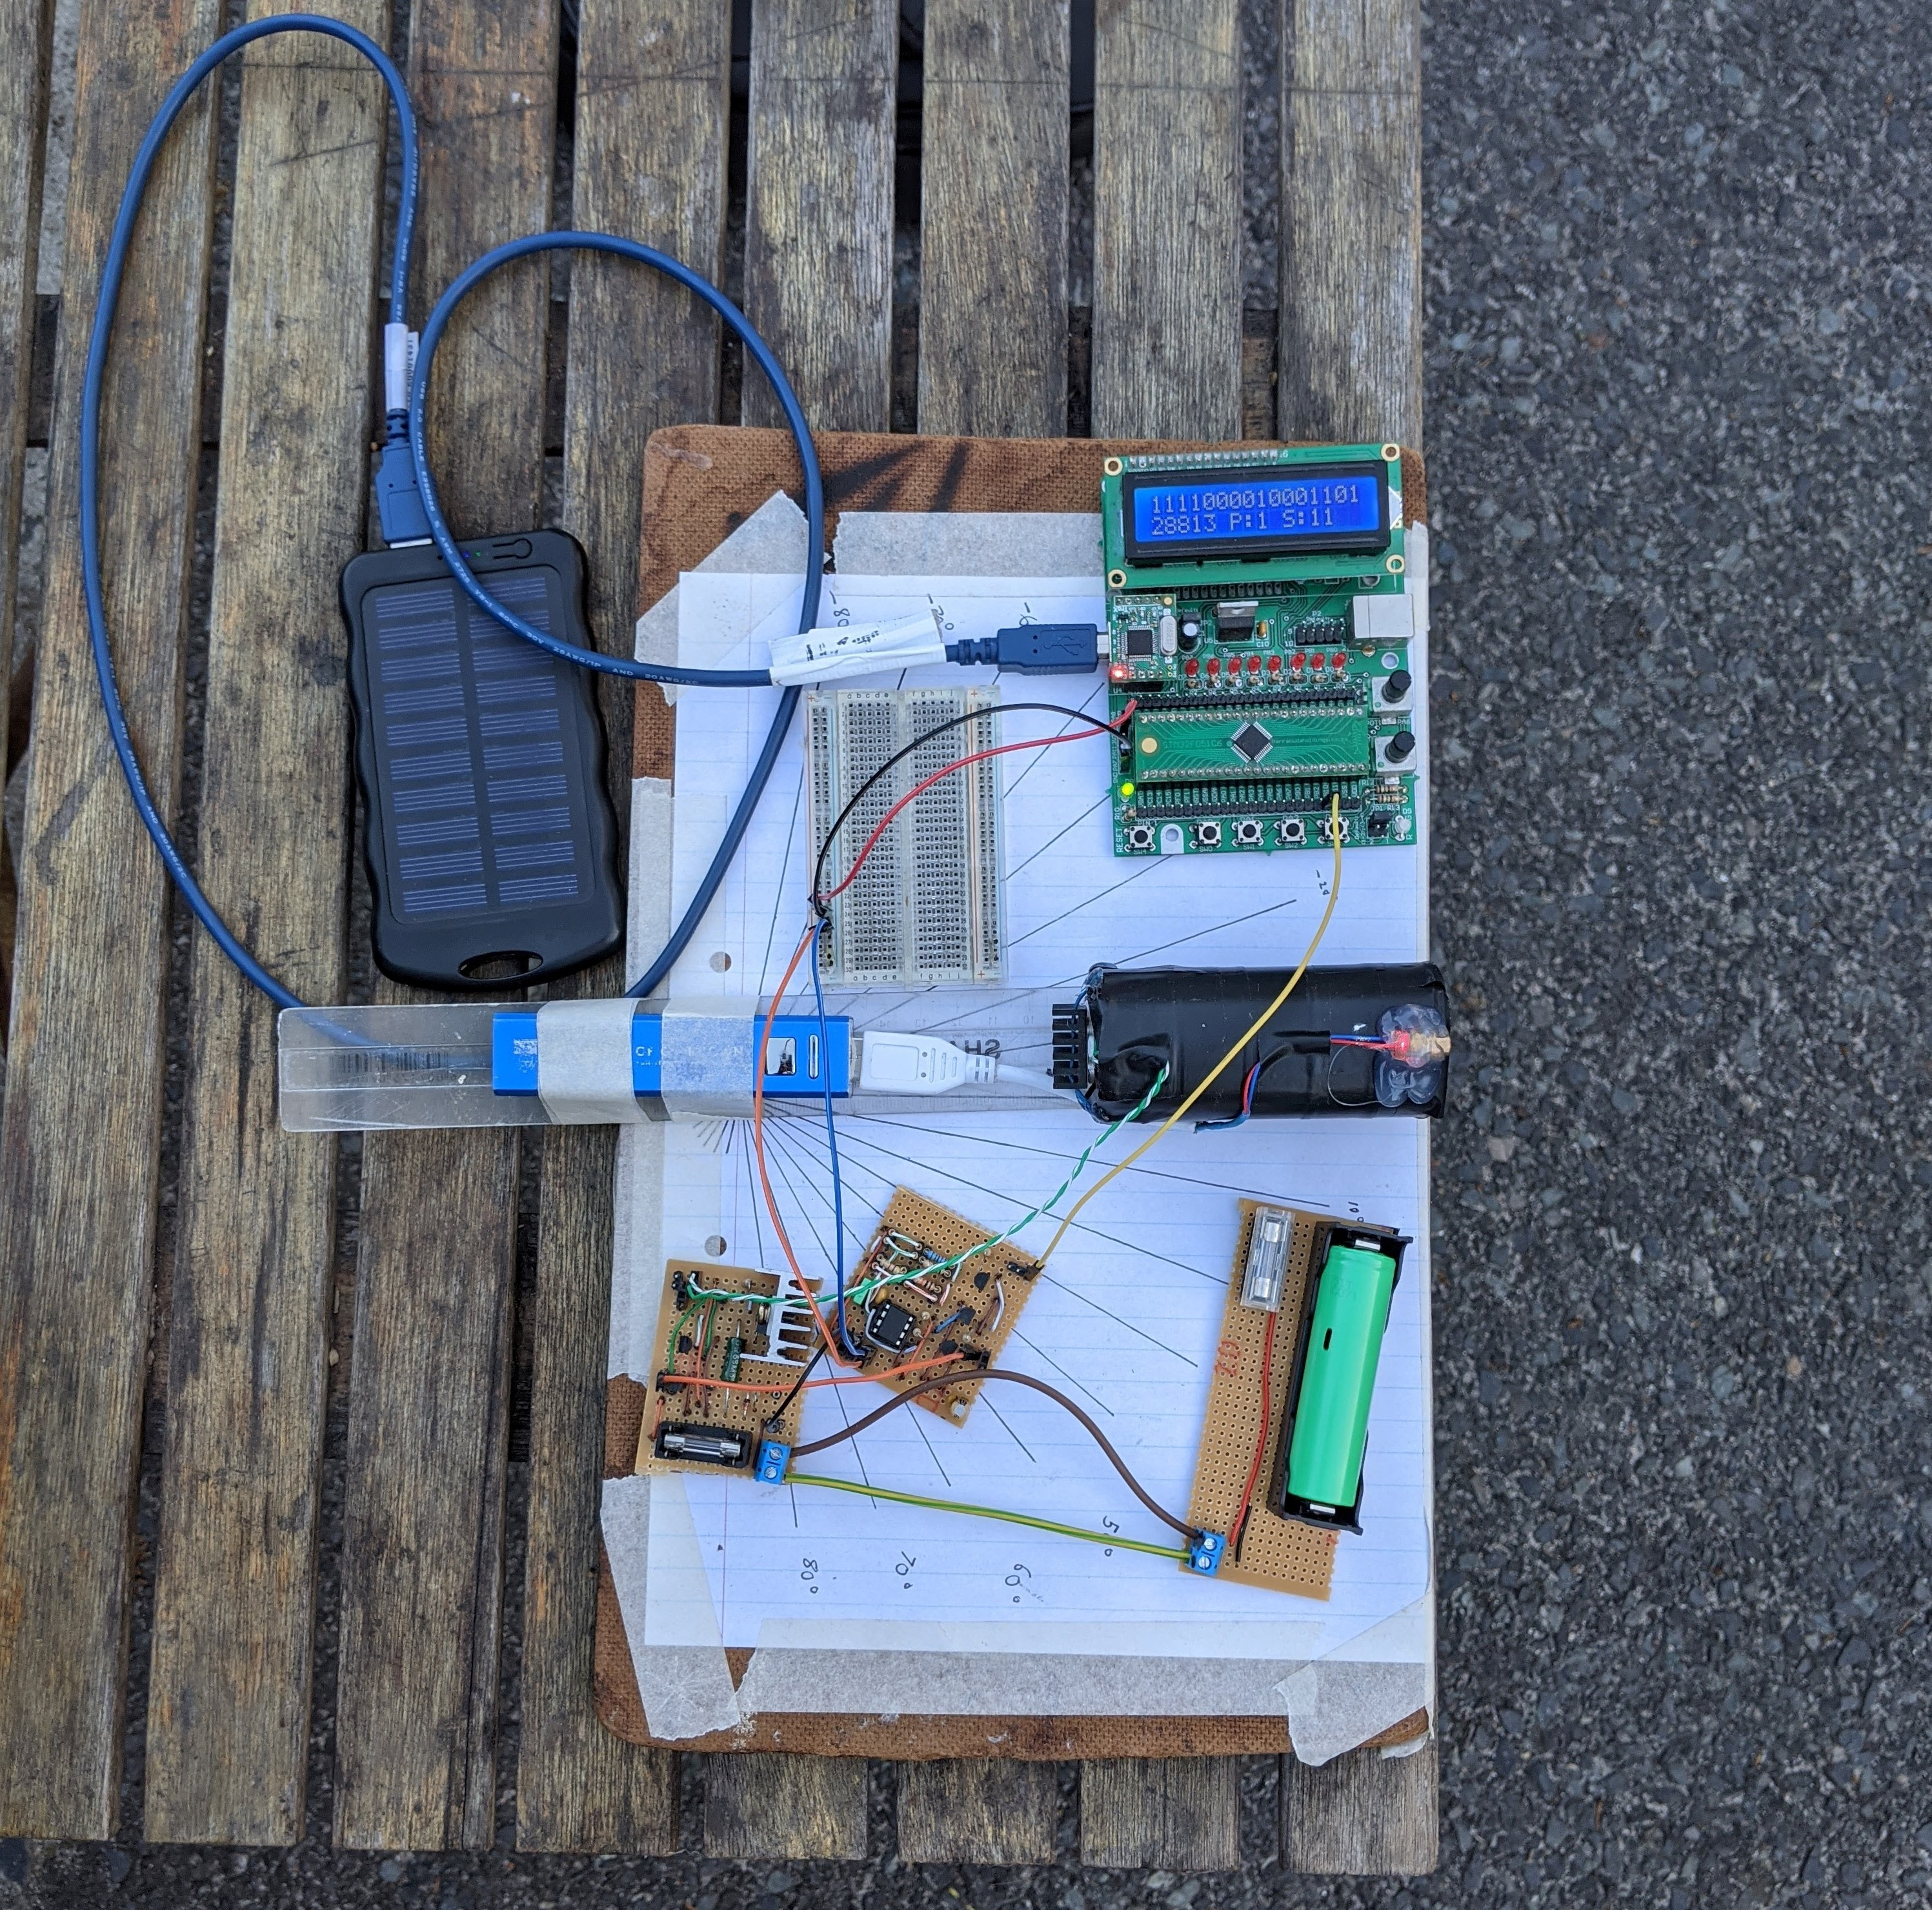
\includegraphics[width=.9\linewidth]{figures/experimentation/transmitter_setup_irl_crop.jpg}
		\captionof{figure}{Tagger Subsystem Experimental Setup}
		\label{fig:transmitter_setup_irl}
	\end{minipage}%
	\hfill
	\begin{minipage}{.48\textwidth}
		\centering
		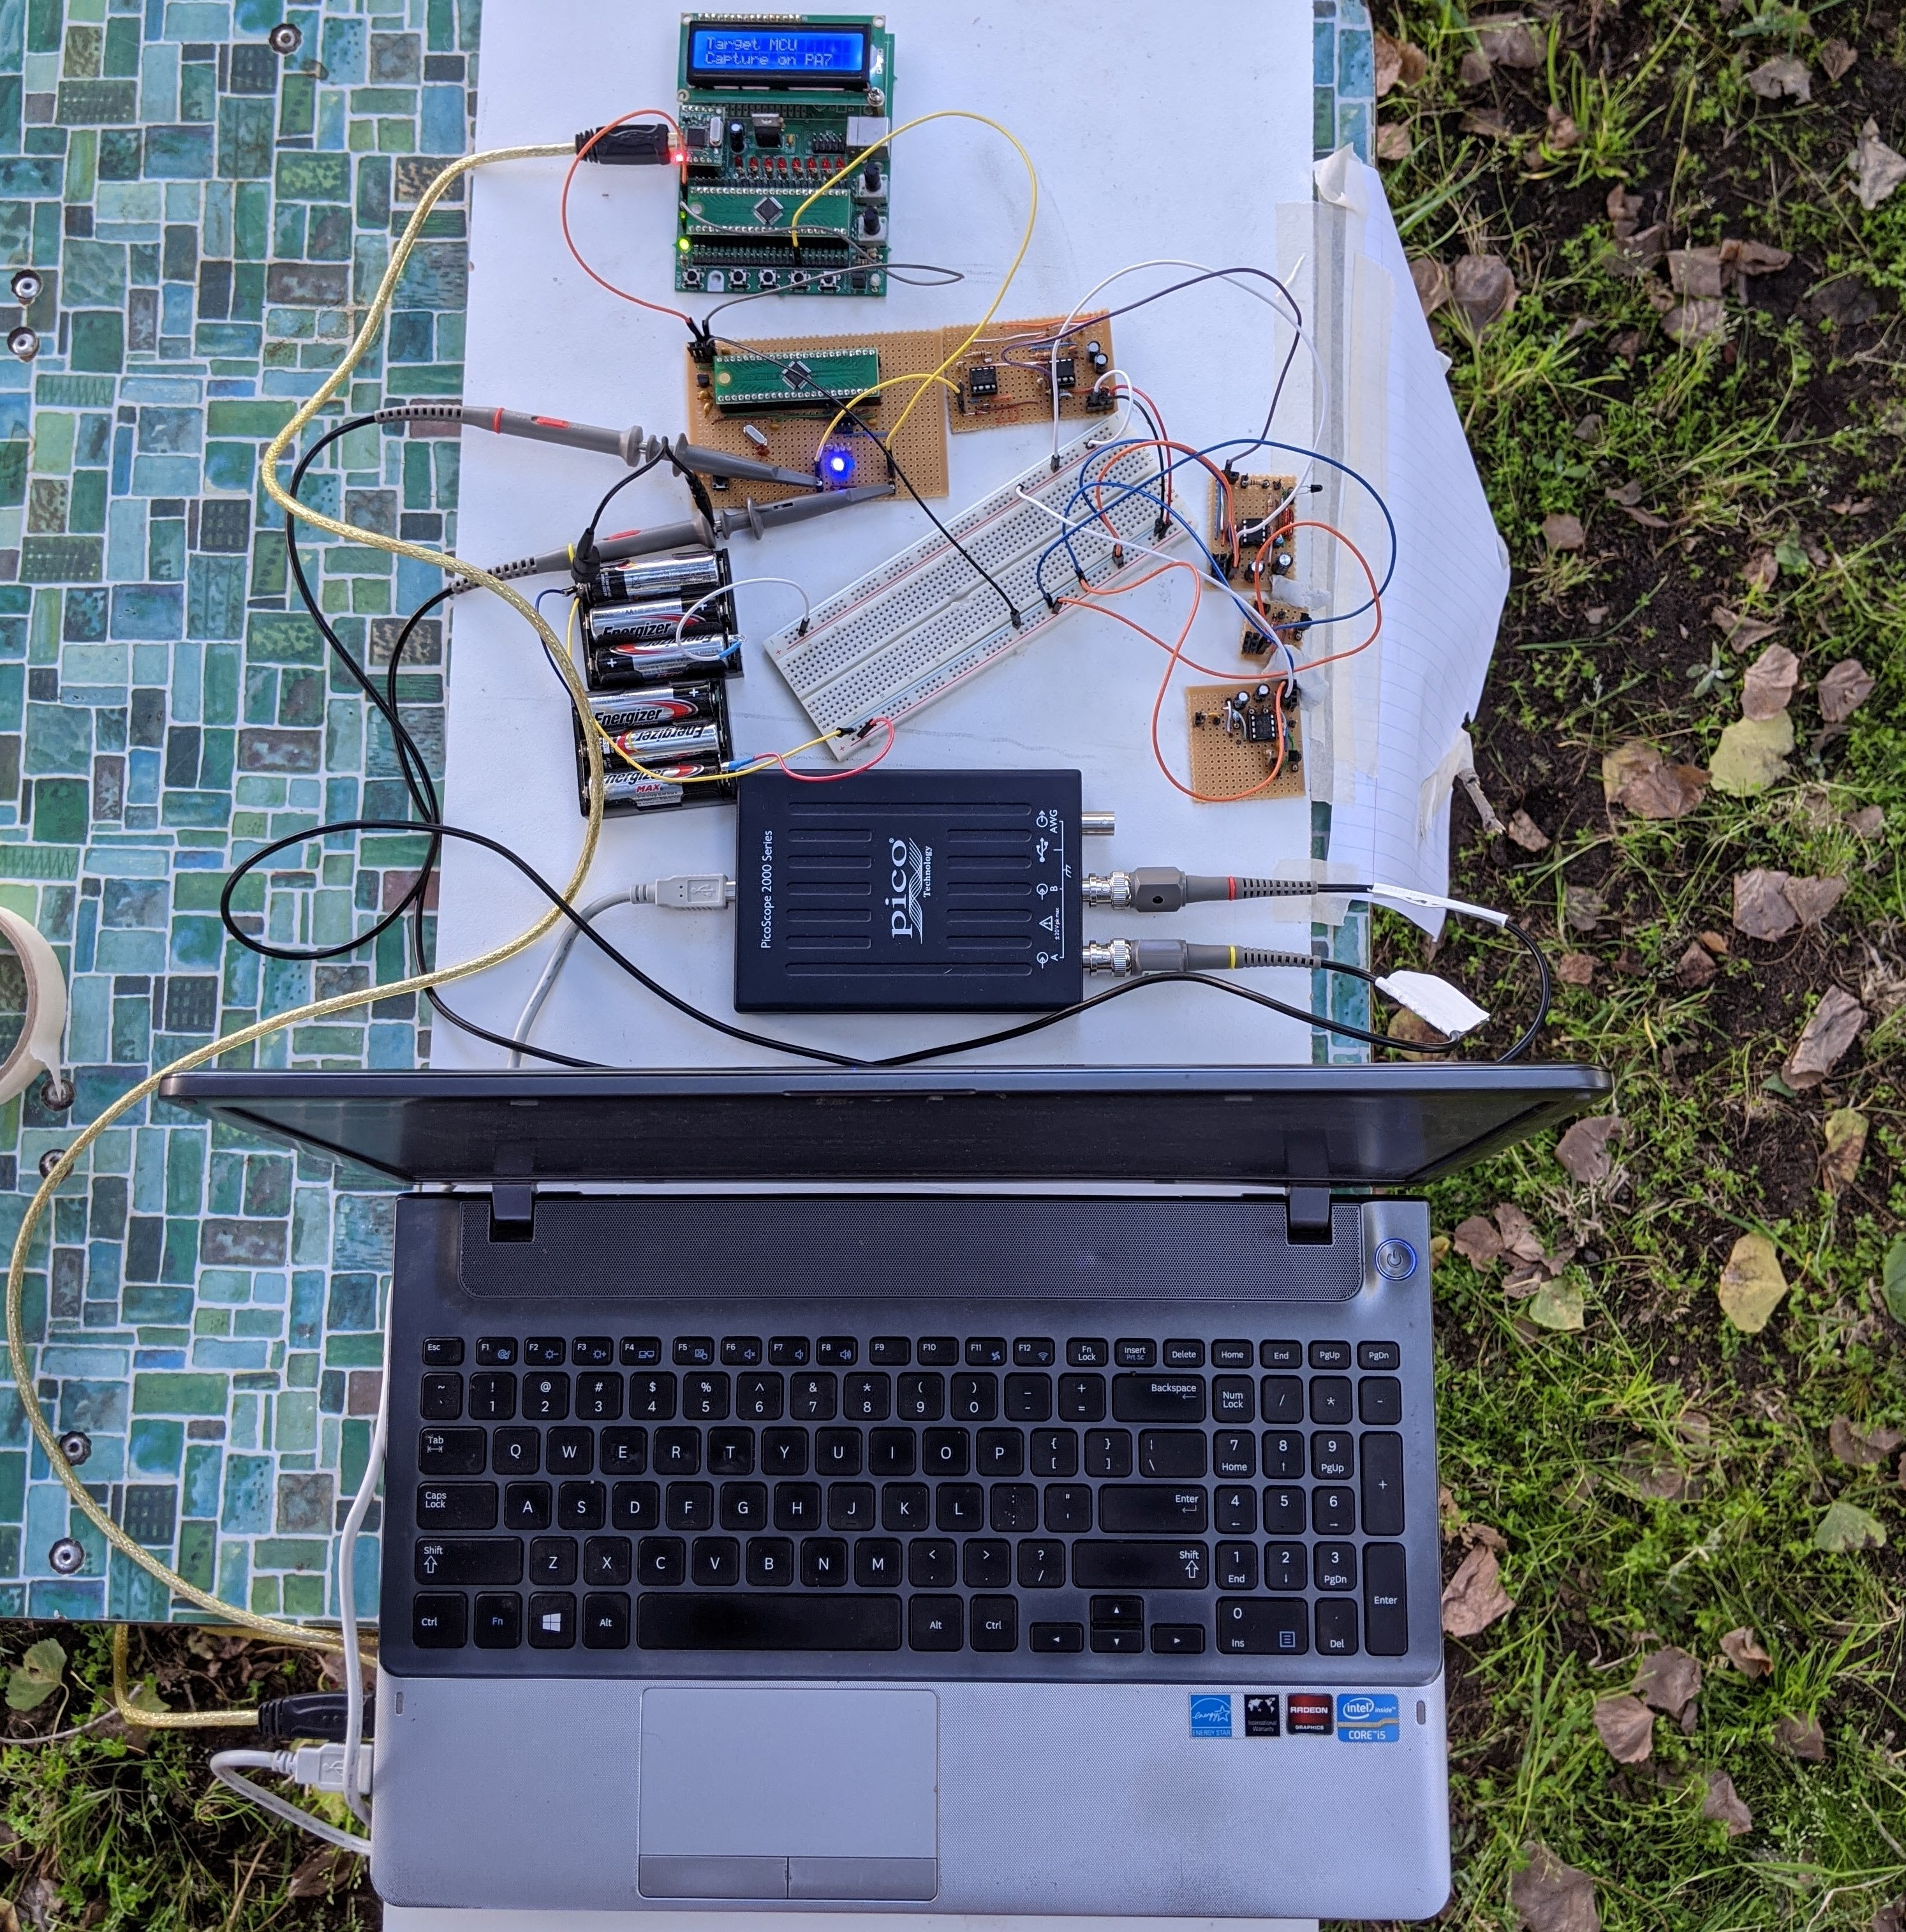
\includegraphics[width=.9\linewidth]{figures/experimentation/receiver_setup_irl_crop.jpg}
		\captionof{figure}{Target Subsystem Experimental Setup}
		\label{fig:receiver_setup_irl}
	\end{minipage}
\end{figure}

Figure \ref{fig:transmitter_setup_irl} and \ref{fig:receiver_setup_irl} show the experimental setup of the tagger and target subsystems respectively.

The range of the system was determined by moving the target subsystem away from the tagger while monitoring the incoming transmissions, the target subsystem was moved until errors began to occur. This was repeated for each of the three detector modules.

The target MCU provided a breakdown of each received transmission and an indicator LED which turned on whenever a transmission was being decoded. When a transmission contained an error the LED indicator would light up but no new transmission data would be displayed. The maximum distance was defined to be the point at which errors would occur, regardless of attempts to align the detector module with the IR beam.

A portable oscilloscope was used to capture waveforms at different locations of the target subsystem. These waveforms were used to investigate the behaviour of the subsystem at the maximum transmission distance.


%%%%%%%%%%%%%%%%%%%%%%%%%%%%%%%%%%%%%%%%%%%
%%%%%%%%%%%%%%%%%%%%%%%%%%%%%%%%%%%%%%%%%%%